در این فصل به طور اجمالی مروری بر پیش‌زمینه‌ی پژوهش انجام شده است. در هر بخش سعی شده است که با حفظ اختصار، تنها جنبه‌های  کاربردی مرتبط با پژوهش مطرح گردد.
\section{مدل بازیگر}

در زمینه‌ی برنامه‌نویسی همروند پژوهش‌های مختلفی صورت گرفته و مدل‌هایی ارائه شده است\cite{Briot98concurrencyand}. در این میان \gls{مدل بازیگر} با توجه به استفاده از ارتباط ناهمگام و قابلیت توزیع بالا توجه زیادی را به خود جذب کرده است. با توجه به ارتباط تنگاتنگ این مدل با پژوهش حاضر، در این بخش به معرفی اجمالی این مدل می‌پردازیم.
لفظ بازیگر برای اولین بار در حدود ۳ دهه پیش توسط هیوئیت  \cite{Hewitt1972} به کار گرفته شد. بازیگر در کاربرد هیوئیت به معنی موجودیت‌های فعالی بود که در یک پایگاه دانش به جستجو پرداخته و در نتیجه کنش‌هایی را ایجاد می‌نمودند. در دهه‌های بعدی گروه هیوئیت با تکیه بر بازیگرها به عنوان عامل‌های محاسباتی\LTRfootnote{agents of computation} مدل بازیگر را به عنوان یک مدل محاسباتی همروند گسترش داد. خلاصه‌ای از تاریخچه‌ی مدل بازیگر در \cite{AghaMST97} موجود است. امروزه برداشت عمومی از مدل بازیگر مربوط به  آقا\cite{Agha_86} می‌باشد. در ادامه‌ی این بخش مشخصات مدل بازیگر ارائه شده است.
 
مدل بازیگر که توسط هیوئیت و آقا \cite{Hewitt1972,Agha1987,Agha1990} ایجاد شده‌است، یک نمایش سطح بالا از سیستم‌های توزیع‌شده فراهم می‌کند. 
\gls{بازیگر}ها
اشیای \gls{لفافه‌بندی‌شده}‌ای هستند که به صورت \gls{همروند} فعالیت می‌کنند و دارای \gls{رفتار}\LTRfootnote{Behavior} قابل تغییر هستند. 
بازیگرها \gls{حالت  مشترک}\LTRfootnote{Shared State} ندارند و تنها راه ارتباط بین آنها تبادل ناهمگام پیغام است. 
 در مدل اکتور فرضی در مورد مسیر پیغام و میزان تاخیر در رسیدن پیغام وجود ندارد، در نتیجه ترتیب رسیدن پیغام‌ها \gls{غیرقطعی} است.
 در یک دیدگاه می‌توان بازیگر را یک \gls{شی‌ء} در نظر گرفت که به یک ریسمان\gls{ریسمان}\LTRfootnote{Thread} کنترل، یک صندوق پست و یک نام غیر قابل تغییر و به صورت سرارسی یکتا \LTRfootnote{Globally Unique} مجهز شده است. برای ارسال پیغام به یک بازیگر، از نام آن استفاده می‌شود. در این مدل، نام  یک بازیگر را می‌توان در قالب پیغام  ارسال کرد. پاسخگویی به هر پیام شامل برداشتن آن پیام از صندوق پستی و اجرای عملیات متناسب با آن است.
این اجرای عملیات به صورت \gls{تجزیه‌ناپذیر}\LTRfootnote{Atomic} و بی‌وقفه خواهد بود\cite{Agha_86}.

\begin{figure*}
    \begin{center}
	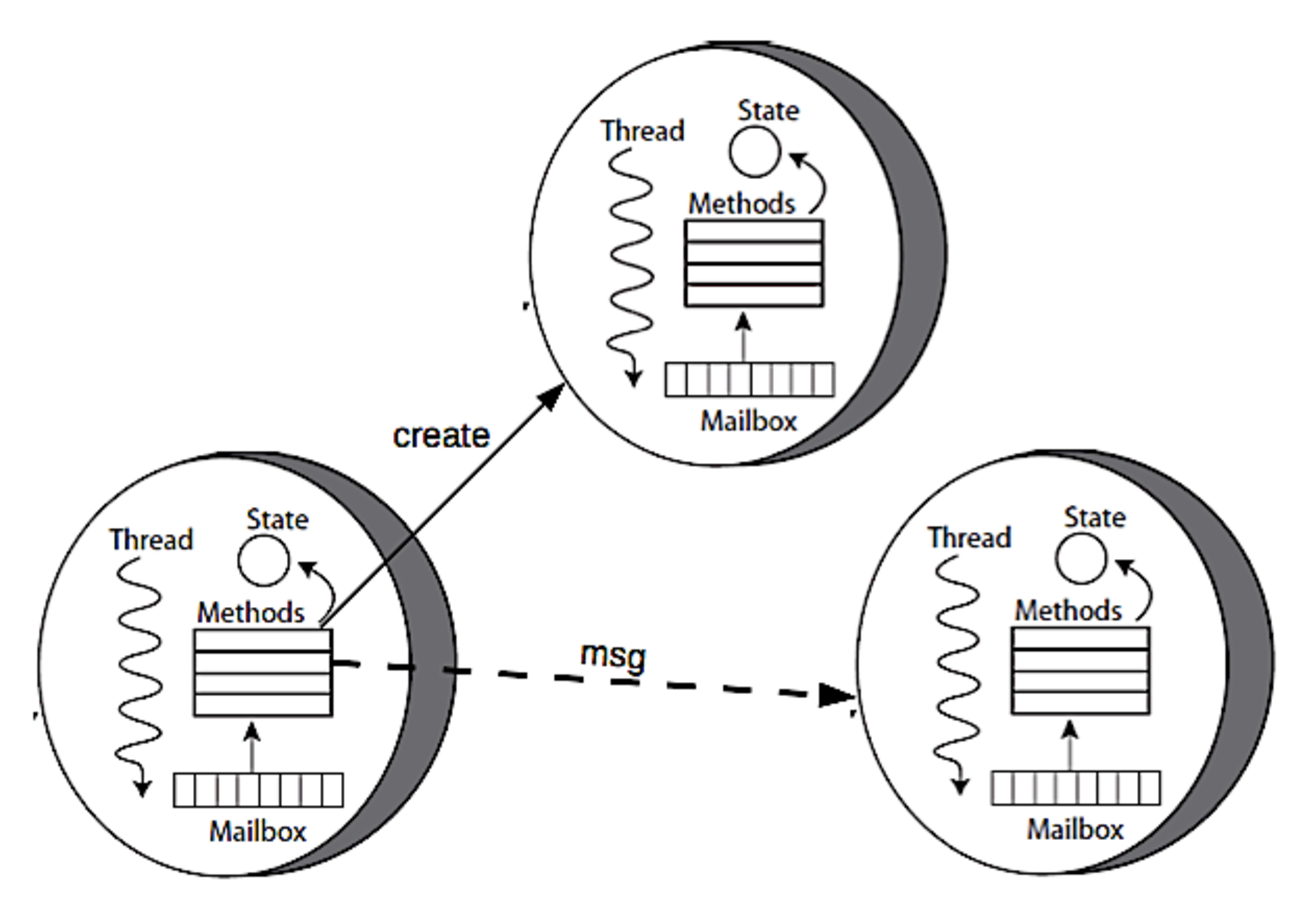
\includegraphics[width=12cm]{2-Preliminaries/Figures/Actor_Structure.pdf}
    \end{center}
    \caption{\label{fig:actorStructure} بازیگر‌ها موجودیت‌های همروندی هستند که به صورت ناهمگام تبادل پیغام انجام ‌می‌دهند. }
\end{figure*}


همان گونه که گفته‌شد، مدل بازیگر سیستم را در سطح بالایی از انتزاع مدل می‌کند.
این ویژگی دامنهٔ سیستم‌های قابل مدلسازی توسط مدل بازیگر را بسیار وسیع نموده‌است.
انواع سیستم‌های سخت‌افزاری و نرم‌افزاری طراحی‌شده برای زیرساخت‌های خاص یا عام، و همچنین الگوریتم‌ها و پروتکل‌های توزیع‌شدهٔ مورد استفاده در شبکه‌های ارتباطی از جملهٔ موارد مناسب برای بهره‌گیری از مدل بازیگر هستند. شکل \ref{fig:actorStructure} شمای کلی از مدل بازیگر و نحوه‌ی تعامل بازیگر‌ها را نشان می‌دهد.
 
 یک بازیگر در نتیجه‌ی دریافت پیغام احتمالا محاسباتی انجام می‌دهد و در نتیجه‌ی آن یک از ۳ عمل زیر را انجام می‌دهد:
\begin{itemize}
\item ارسال پیغام به سایر بازیگر‌ها
\item ایجاد بازیگر جدید
\item تغییر حالت محلی
\end{itemize} 

\subsection{\gls{معناشناسی}}\LTRfootnote{Semantics}
از نظر معناشناسی مشخصه‌های کلیدی مدل محض بازیگر عبارتند از: لفافه‌بندی و
  \gls{تجزیه‌ناپذیر}‌ی\LTRfootnote{Encapsulation and Atomicity}، \gls{انصاف}\LTRfootnote{Fairness}، 
  استقلال از مکان\LTRfootnote{Location Transparency}، توزیع\LTRfootnote{Distribution} و تحرک\LTRfootnote{Mobility}
 \cite{KarmaniAgha_Actors_11}. 
  باید توجه داشت که این مشخصه‌ها در مدل محض  وجود دارند و این الزاما به این معنی نیست که تمام زبان‌های مبتنی بر مدل بازیگر از این مشخصه‌ها پشتیبانی می‌کنند. ممکن است تعدادی از این مشخصه‌ها در  زبان‌های مبتنی بر بازیگر  با در نظر گرفتن اهدفی مانند کارایی و سهولت پیاده‌سازی نشده‌اند. در این موارد باید با به کار بردن ابزار‌های بررسی ایستا، مترجم‌ها و یا با تکیه بر عملکرد درست برنامه‌نویس از صحت عملکرد برنامه‌ اطمینان حاصل کرد \cite{ActorsJVM2009}. 
\begin{itemize}
\item \textbf{لفافه‌بندی و \gls{تجزیه‌ناپذیر}ی:}\LTRfootnote{Encapsulation and Atomicity}  
نتیجه‌ی مستقیم مشخصه‌ی لفافه‌بندی در بازیگر‌ها این است که درهیچ دو بازیگری، به اشتراک گذاری حالت وجود ندارد. این مشخصه، \gls{تجزیه}ی \gls{شیءگونه}ی برنامه را تسهیل می‌کند. در زبان‌های برنامه‌نویسی \gls{شیء-بنیاد} مشخصه منجر به ایجاد تغییر تجزیه‌ناپذیر شده است. به این صورت که وقتی یک شیء، شیء دیگری را فراخوانی می‌کند، شیء مقصد تا پایان محاسبات مربوط به این فراخوانی، به فراخوانی‌های دیگر پاسخ نمی‌دهد.  این مشخصه به ما اجازه می‌دهد تا بتوانیم در باره‌ی رفتار یک شیء در قبال دریافت یک پیغام (فراخوانی) با توجه به حالت شیء در زمان دریافت آن \gls{استدلال} کنیم.

در محاسبات همروند، وقتی یک بازیگر مشغول انجام محاسبات مربوط به یک پیغام است، امکان دریافت پیغام جدید توسط آن وجود دارد اما مشخصه‌ی تجزیه‌ناپذیری تضمین می‌کند که پیغام جدید امکان قطع محاسبات جاری بازیگر و تغییر حالت محلی آن را ندارد. این مشخصه الزام می‌کند که بازیگر گیرنده، در هر لحظه فقط یک پیغام در حال پردازش داشته باشد و محاسبات مربوط به  پیغام جاری را در یک قدم بزرگ\LTRfootnote{Macro-Step} به صورت تجزیه ناپذیر طی کند. \cite{AghaMST97}
مشخصه‌های معناشناسی لفافه‌بندی و تجزیه ناپذیری به طور  چشم‌گیری از عدم قطعیت مدل بازیگر می‌کاهند و با کوچکتر کردن فضای حالت برنامه‌های نوشته شده در مدل بازیگر، این برنامه‌ها را برای استفاده در ابزارهای آزمون درستی و  verification(?) قابل استفاده می‌کند\cite{LauterburgKMA10}.
این دو مشخصه مجموعا باعث می‌شوند تا بتوانیم بر اساس پیغام انتخاب شده برای اجرا و وضعیت محلی بازیگر در هنگام شروع به اجرا ، رفتار یک بازیگر قابل پیش‌بینی باشد.

\item \textbf{ \gls{انصاف}:}
انصاف در مدل بازیگر به این مفهوم است که پیغام فرستاده شده نهایتا به بازیگر مقصد خواهد رسید، مگر آنکه بازیگر مقصد به طور دائمی غیر فعال شده باشد. لازم به ذکر است که این تعریف از  انصاف در رسیدن پیغام به بازیگر مقصد، متضمن انصاف در \gls{زمان‌بندی} بازیگر‌ها است. به این مفهوم که در صورتی که یک بازیگر در اثر  زمان‌بندی غیر منصفانه، موفق به اخذ نوبت اجرا نشود، پیغام‌های فرستاده شده به مقصد آن بازیگر هرگز به مقصد نخواهند رسید. انصاف علاوه بر تضمین رسیدن پیغام‌ها، امکان استدلال مناسب درباره‌ی نحوه‌ی تداوم اجرای  برنامه‌\LTRfootnote{Liveness Property} را فراهم می‌کند. میزان طبیعتا میزان موفقیت در تضمین این مشخصه در محیط‌های مبتنی بر بازیگر وابسته به منابع موجود در سیستم در حال اجرا است \cite{ActorsJVM2009}.
\item \textbf{ استقلال از مکان، توزیع و تحرک:}
\label{mobility}
در مدل بازیگر، ارسال پیغام به یک بازیگر تنها از طریق دسترسی به نام آن بازیگر ممکن می‌شود. مکان واقعی بازیگر تأثیری روی نام آن ندارد. هر بازیگر دارای فضای آدرس مربوط به خود است که می‌تواند کاملا متفاوت با دیگر بازیگر‌ها باشد. بازیگرهایی که به یکدیگر پیغام می‌فرستند می‌توانند روی یک هسته از یک پردازنده‌ی مشترک اجرا شوند یا اینکه در ماشین دیگری که از طریق شبکه به آنها مرتبط می‌شوند در حال اجرا باشند. مشخصه‌ی  استقلال از مکان در مدل بازیگر به برنامه‌نویس این امکان را می‌دهد که فارغ از نگرانی درباره‌ی محل اجرای  بازیگر ها به برنامه‌نویسی بپردازد.
 عدم اطلاع از مکان اجرای بازیگران  منجر به قابلیت حرکت در آنها می‌شود. تحرک به صورت قابلیت انتقال پردازش به نودهای دیگر تعریف می‌شود.در سطح سیستم، تحرک از جهت توزین بار \LTRfootnote{Load-Balancing}، قابلیت تحمل خطا\LTRfootnote{Fault Tolerance} و نیز پیکربندی مجدد\LTRfootnote{Reconfiguration} حائز 
 اهمیت است.
 پژوهش‌های پیشین نشان می‌دهد که قابلیت تحرک در رسیدن به کارایی \gls{مقیاس‌پذیر} به ویژه در کاربردهای  \gls{بی‌قاعده}\LTRfootnote{Irregular} روی ساختار داده‌های \gls{پراکنده} مفید است\cite{KimA95}. در کاربردهای دیگر، توزیع بهینه به شرایط زمان اجرا و میزان بار وابسته است. به عنوان مثال، در کاربردهای وب، تحرک با توجه به شرایط شبکه و امکانات کلاینت مورد استفاده قرار می‌گیرد\cite{ContextAwareWeb}.  
از سوی دیگر، قابلیت تحرک می‌تواند در کاهش انرژی مصرفی در اثر اجرای کاربردهای موازی مفید باشد. در این کاربردها، محاسبات موازی به صورت پویا بین تعداد هسته‌های بهینه (تعداد هسته‌هایی که منجر به کمترین مصرف می‌شوند) توزین می‌شوند. قسمت‌های مختلف یک کاربرد می‌تواند شامل الگوریتم‌های موازی مختلفی باشد و میزان مصرف انرژی یک الگوریتم به تعداد هسته‌های مشغول اجرای الگوریتم و نیز بسامد اجرای آن هسته‌ها بستگی دارد\cite{KorthikantiA10}. در نتیجه، ویژگی تحرک پذیری بازیگر‌ها، ویژگی مهمی برای برنامه نویسی در معماری‌های چند-هسته‌ای به شمار می‌آید.

\end{itemize} 


\subsection{پیاده‌سازی‌ها}
\label{subsection:actorImpls}
برای مدل بازیگر زبان‌ها و چارچوب‌های زیادی توسعه داده شده است. ABCL، POOL، ConcurrentSmalltalk، ACT++ و CEiffel تعدادی از پیاده‌سازی‌های اولیه از این مدل می‌باشند. مرجع \cite{Briot98concurrencyand} به بررسی این زبان‌ها پرداخته است. شاید بتوان زبان  \gls{ارلانگ}\LTRfootnote{Erlang}\cite{erlang} را معروفترین پیاده‌سازی مدل بازیگر دانست. این زبان در حدود ۲۲ سال قبل برای برنامه‌نویسی سوئیچ‌های مخابراتی شرکت اریکسون\LTRfootnote{Ericsson} توسعه داده شد. علاوه بر ارلانگ زبان‌ها و چارچوب‌های مبتنی بر مدل بازیگر دیگری نیز در سال‌های اخیر مورد استفاده گرفته‌اند که کتابخانه‌ی بازیگر اسکالا
\LTRfootnote{Scala Actor Library} \cite{ScalaActors}،  Ptolemy \cite{Ptolemy}، SALSA \cite{salsa}، CHARM++ \cite{CHARMplus}، ActorFoundry \cite{ActorFoundry}، Asynchronous Agents Library \cite{AsyncAgentsLib}  از جمله‌ی آنها هستند.
  از کاربردهای متن-باز که بر مبنای مدل بازیگر توسعه داده شده‌اند می‌توان به سیستم تبادل پیغام توئیتر\LTRfootnote{Twitter} و چارچوب تحت وب لیفت\LTRfootnote{Lift} و از میان کاربرد‌های تجاری می‌توان به سیستم گپ\LTRfootnote{Chat} فیسبوک و موتور بازی وندتا\LTRfootnote{Vendetta game engine} اشاره کرد.
در این پژوهش برای پیاده‌سازی نسخه‌ی مبتنی بر تبادل ناهمگام پیغام از کتابخانه‌ی بازیگر اسکالا استفاده شده است (چرا؟) که در بخش ؟ معرفی شده است.


\section{معرفی زبان اسکالاو  کتابخانه‌بازیگر اسکالا}
\label{section:Scala}
همان طور که در بخش \ref{subsection:actorImpls} اشاره شد، پیاده‌سازی‌های مختلفی از مدل بازیگر در زبان‌ها و چارچوب‌های برنامه‌نویسی ارائه شده است. مقاله‌ی \cite{ActorsJVM2009} به بررسی و مقایسه‌ی این پیاده‌سازی‌ها پرداخته است. در این پژوهش زبان اسکالا و کتابخانه‌ی بازیگر آن برای پیاده‌سازی مطالعه‌ی موردی انتخاب شده است. گستردگی ابزار و همچنین فعال بودن جامعه\LTRfootnote{Community}‌ی برنامه‌نویسی این زبان اصلی‌ترین انگیزه‌های انتخاب این زبان برای پیاده‌سازی بوده‌اند. ضمنا با توجه به انتخاب زبان جاوا برای پیاده‌سازی نسخه‌ی متداول مورد مطالعه و ارتباط تنگاتنگ زبانهای اسکالا و جاوا، انتخاب زبان اسکالا منجر به سهولت ارزیابی مقایسه‌ای مطالعه‌ی موردی شده است. در این بخش به معرفی اجمالی زبان اسکالا و کتابخانه‌ی بازیگر آن پرداخته شده است. هدف از این معرفی، سهولت درک روش طراحی پیشنهادی در فصل ۳ می باشد و به همین دلیل از توضیح جزئیات و امکانات اضافی این زبان خودداری شده است. کتاب \cite{programmingInScala} به عنوان منبع این بخش استفاده شده است.
\subsection{زبان اسکالا}
اسکالا مخفف عبارت \emph{''زبان مقیاس‌پذیر``}\LTRfootnote{Scalable Language} است و اشاره به این نکته دارد که اسکالا برای رشد بر اساس نیاز کاربر طراحی شده است. اسکالا را می‌توان برای گستره‌ی وسیعی از کاربردها از نوشتن اسکریپت‌های کوچک گرفته تا پیاده‌سازی سیستم‌های بزرگ به کار برد. برنامه‌های اسکالا بر روی محیط اجرایی جاوا\LTRfootnote{JRE}  قابل اجرا هستند و در برنامه‌های اسکالا  می‌توان از کتابخانه‌های استاندارد جاوا استفاده کرد.
زبان اسکالا ترکیبی از ویژگی‌های زبان‌های \gls{تابعی} و شیءگرا را در خود دارد. در زبان‌های تابعی، توابع مانند انواع داده‌ها قابل ارجاع هستند. اسکالا مانند جاوا دارای \gls{بررسی گونه‌ها}ی، \gls{ایستا} است.
\codelisting[language=scala]{2-Preliminaries/src/Sample.scala}{قطعه کد نمونه برای زبان اسکالا}{figure:scalaSample}

در ادامه مشخصات نحوی زبان اسکالا در قالب یک مثال توضیح داده می‌شود. در شکل \ref{figure:scalaSample} قطعه کد اسکالا مربوط به کلاس Course نمایش داده شده است. برای آشنایی با نحو زبان اسکالا به بررسی این کد می‌پردازیم:\\
در خطوط ۱و ۲ کلاس Course و متغیرهای ،id ،name units و prerequisites به عنوان فیلد‌های آن تعریف شده‌اند. در خط ۴ تابع equals از این کلاس override شده است. در اسکالا همانند جاوا هر کلاس به طور پیش‌فرض دارای یک تابع‌ equals است که در صورت لزوم می‌توان آن را override کرد. همان‌طور که در کد مشخص است، تعریف تابع در اسکالا با کلمه‌ی کلیدی  \textbf{def} انجام می‌گیرد. در خطوط ۴ تا ۸ شرط لازم برای یکسان بودن یک شیء از نوع Course با شیء حاضر پیاده‌سازی شده است. نوع و مقدار یک متغیر را می‌توان با استفاده از دستور \lr{match .. case .. } با انواع و مقادیر دلخواه مقایسه کرد. نتیجه‌ی دستورات خطوط ۶ و ۷ این است که اگر متغیر other از نوع Course باشد و مقدار فیلد id آن با مقدار فیلد id از شیء حاضر یکسان باشد تابع مقدار true را برمی‌گرداند. خط ۸ به این معنا است که اگر هر حالت دیگری به جز حالت قبل بود مقدار false برگردانده ‌می‌شود. در خط ۱۲ ‌نمونه‌ای از حلقه‌ی for نمایش داده شده است. در اسکالا حلقه‌ها به صورت‌های متنوعی می‌توانند بیان شوند که در این مثال یک حالت از آنها نمایش داده شده است.  در خط ۱۲ متغیر pre برای گرفتن مقدار موقت حلقه تعریف شده است. نکته‌ی جالب توجه این است که در این خط، نوع متغیر تعریف نشده است. در بخش قبل ذکر شد که اسکالا دارای خاصیت بررسی گونه‌های ایستا \LTRfootnote{static type checking} است. ظاهرا این دو امر در تناقض با یکدیگر هستند اما باید توجه داشت که در زبان اسکالا نوعی از استنتاجِ گونه\LTRfootnote{type inference} در زمان ترجمه اتفاق می‌افتد. در این مورد با توجه به اینکه متغیر pre از لیست prerequisites مقداردهی می‌شود، گونه‌ی آن در زمان ترجمه قابل استنتاج است. خط ۱۶ تابع دیگری را نشان می‌دهد که در آن تابع toString، override شده است. نکته‌ی قابل توجه در مورد این قسمت از کد عدم استفاده از علامت \{ \} برای تعیین حوزه‌ی تابع است. در زبان اسکالا به دلیل وجود ویژگی‌های زبان‌های تابعی، می‌توانیم با توابع مانند متغیر‌ها و داده‌ها رفتار کنیم که این بخش از کد مثالی از این ویژگی است. همانطور که در این مثال مشخص است، در زبان اسکالا استفاده از نقطه‌ویرگول (;) در اکثر موارد اختیاری است.

\subsection{کتابخانه‌ی بازیگر اسکالا}
همانطور که در بخش \ref{subsection:actorImpls} اشاره شد، یکی از پیاده‌سازی‌های مدل بازیگر، کتابخانه‌ی بازیگر اسکالا است. در این بخش به معرفی اجمالی کتابخانه‌ی بازیگر اسکالا و طرز استفاده از آن برای برنامه‌نویسی همروند می‌پردازیم.
\subsubsection{ایجاد بازیگر}
بازیگر‌ها در اسکالا از کلاس scala.actors.Actor مشتق می‌شوند.  شکل \ref{figure:sillyActor} کد مربوط به  یک بازیگر ساده را نشان می‌دهد. این بازیگر کاری به صندوق پیغام‌ها ندارد و صرفا پنج بار پیغام \lr{I'm acting!} را چاپ می‌کند و سپس اجرای آن خاتمه می‌یابد.

\codelisting[language=scala]{2-Preliminaries/src/SillyActor.scala}{کد یک بازیگر ساده در زبان اسکالا}{figure:sillyActor}

  بازیگر‌ها در اسکالا با دستور start() شروع به فعالیت می‌کنند. با شروع به فعالیت یک بازیگر، تابع act() آن فراخوانی می‌شود و تا زمانی که اجرای این تابع به اتمام نرسد، بازیگر به طور همروند در حال اجرا باقی می‌ماند. در صورتی که بخواهیم بازیگر به طور دائمی در حال اجرا بماند دو راه وجود دارد. راه اول این است که تابع act() را در پایان کار  خود مجدداً فراخوانی کنیم. و راه دیگر استفاده از عبارت \textbf{loop} در اسکالا است. دستورات درون حلقه‌ی loop به صورت بی‌پایان اجرا می‌شوند. شکل \ref{fig:endlessActor} کدهای مربوط به این ۲ روش را نمایش می‌دهد.

\begin{figure*}
    \begin{center}
    \begin{tabular}{ c  c }
      	%\hline
	 & \\

	\begin{latin}
\linespread{1.1}
\lstinputlisting[language=scala]{2-Preliminaries/src/SillyActor2.scala}
\end{latin} & 
 \begin{latin}
	\linespread{1.1}
	\lstinputlisting[language=scala]{2-Preliminaries/src/SillyActor3.scala}
\end{latin}
 	\\
         (الف) & (ب) \\
%	\hline
    \end{tabular}
    \end{center}
    \caption{\label{fig:endlessActor} تداوم اجرای بازیگر با استفاده از الف)فراخوانی بازگشتی و ب)حلقه‌ی loop}
\end{figure*}


\subsubsection{تبادل پیغام}
عملگر \textbf{!} برای فرستادن پیغام ناهمگام استفاده می‌شود. دستور \lr{dest ! message} پیغام message را برای بازیگر dest ارسال می‌کند بدون آنکه برای دریافت جواب منتظر بماند. با اینکه در مدل اکتور دستوری برای تبادل همگام پیغام وجود ندارد، در اکثر پیاده‌سازی‌ها این امکان به مدل اضافه شده است\cite{ActorsJVM2009}. در کتابخانه‌ی بازیگر اسکالا، عملگر \lr{!?} به این منظور به کار گرفته می‌شود. در صورت استفاده از این دستور، فرستنده‌ی پیغام تا گرفتن جواب متوقف می‌ماند. برای برداشتن پیغام از صندوق پیغام‌ها، از دستور receive استفاده می‌شود. شکل \ref{fig:pingPongActor} مثالی از نحوه‌ی تبادل پیغام بین بازیگران را نمایش می‌دهد. در این برنامه دو بازیگر PingActor و PongActor به تبادل پیغام می‌پردازند. در ابتدا بازیگر PingActor که متغیر آن با مقدار ۱۰۰ مقداردهی شده است یک پیغام Ping برای بازیگر PongActor می‌فرستد و در ادامه در یک حلقه‌ی loop منتظر پاسخ Pong می‌ماند. بازیگر PongActor با گرفتن هر پیغام Ping پاسخ Pong را برای فرستنده ارسال می‌کند. کلمه‌ی کلیدی \textbf{sender} در کلاس Actor اشاره‌گری به فرستنده‌ی پیغام در حال پردازش ‌می‌باشد (خط ۶ از کد قسمت (ب) شکل \ref{fig:pingPongActor}). بازیگر PingActor با دریافت پاسخ‌ Pong مقدار متغیر pingsLeft را چک می‌کند و در صورت مثبت بودن آن پیغام Ping بعدی را ارسال می‌کند و در غیر این صورت پیغام Stop را ارسال ‌می‌کند. نهایتا با صفر شدن متغیر pingsLeft، بازیگر PingActor پیغام Stop را برای PongActor می‌فرستد. دستور exit که در پایان کار هر دو بازیگر استفاده شده است باعث می‌شود ریسمان اجرایی بازیگر رها شود و پس از اجرای این دستور بازیگر قادر به دریافت پیغام نخواهد بود.

\begin{figure*}
    \begin{center}
    \begin{tabular}{ c }
 \begin{latin}
	\linespread{1.1}
	\lstinputlisting[language=scala]{2-Preliminaries/src/Ping.scala}
\end{latin}
\\ 
\scriptsize{(الف) بازیگر Ping که فرستنده‌ی اولیه‌ی پیغام است}
&
\hline
\\
\begin{latin}
\linespread{1.1}
\lstinputlisting[language=scala]{2-Preliminaries/src/Pong.scala}
\end{latin}  
\\
\scriptsize{(ب) بازیگر Pong که به پیغام ping پاسخ می‌دهد.}
          &
\hline
\begin{latin}
\linespread{1.1}
\lstinputlisting[language=scala]{2-Preliminaries/src/PingPong.scala}
\end{latin} 
\\
\scriptsize{(ج) کد اجرای برنامه‌ی PingPong}
         &
\hline

\end{tabular}
\end{center}
\caption{\label{fig:pingPongActor} مثالی از نحوه‌ی تبادل پیغام بین بازیگر‌ها}
\end{figure*}

\subsubsection{بستر اجرای بازیگر‌ها}
event based actors ...